\documentclass{../source/Experiment}

\major{信息工程}
\name{姚桂涛}
\title{A4 倒计时定时器设计、制作与调试}
\stuid{3190105597}
\college{信息与电子工程学院}
\date{\today}
\lab{东4-216}
\course{电子电路设计实验}
\instructor{李锡华、施红军、叶险峰}
\grades{}
\expname{倒计时定时器设计、制作与调试}
\exptype{研究实验}
\partner{郭含蕾}

\begin{document}
    \makecover
    \makeheader
    \section{实验目的}
        \begin{enumerate}
            \item 学习掌握用Arduino UNO 设计倒计时定时器
            \item 学习掌握PCB 电路板的设计和制作
            \item 学习掌握Arduino UNO 扩展板的设计与制作
            \item 学习掌握旋转编码器的使用
        \end{enumerate}
    \section{实验设计任务}
        \begin{enumerate}
            \item 用Arduino UNO 设计倒计时定时器,要求如下:设定倒计时时间若干(设定标准时间数组),通过旋转编码器选择,时间到时报警。
            \item 设计电路,完成相应器件的选择,制作Arduino UNO 扩展板。
            \item 编制与调试倒计时定时器程序。
            \item 将制作的扩展板与Arduino UNO 板组装后,进行系统联调。
        \end{enumerate}
    \section{主要仪器设备}
    Arduino UNO及其扩展版、旋转编码器、七段数码管、蜂鸣器、电阻若干、PNP三极管。
    \section{实验原理}
    本项目使用Arduino UNO 与其扩展板来实现倒计时定时器。下面对各部分模块进行说明。
        \subsection{旋转编码器}
        旋转编码器会游A、B两个输出,当不同方向转动旋转编码器的时候,可以通过A、B信号的不同变化进行区分。同时,旋转编码器还有一个开关输出。
        \subsection{7段数码管}
        7段数码管一般由8个发光二极管组成,其中由7个细长的发光二极管组成数字显示,另外一个圆形的发光二极管显示小数点。发光二极管的阳极连在一起的称为共阳极数码管,阴极连在一起的称为共阴极数码管。

        当发光二极管导通时,相应的一个点或一个笔画发光。控制相应的二极管导通,就能显示出各种字符。

        7段数码管有两种驱动显示方法,一个是静态显示驱动,一个是动态显示驱动。

        静态驱动也称直流驱动。静态驱动是指每个数码管的每一个段码都由一个单片机的I/O脚进行驱动,或者使用如BCD 码二-十进位计数器进行驱动。静态驱动的优点是编程简单,显示亮度高,缺点是占用I/O 脚多。

        动态驱动是将所有数码管的8 个显示笔划"a,b,c,d,e,f,g,dp "的同名端连在一起,另外为每个数码管的公共极COM 增加位元选通控制电路,位元选通由各自独立的I/O 线控制,当单片机输出字形码时,所有数码管都接收到相同的字形码,但究竟是那个数码管会显示出字形,取决于单片机对位元选通COM 端电路的控制,所以我们只要将需要显示的数码管的选通控制打开,该位元就显示出字形,没有选通的数码管就不会亮。

        透过分时轮流控制各个LED 数码管的COM 端,就使各个数码管轮流受控显示,这就是动态驱动。在轮流显示过程中,每位元数码管的点亮时间为1~2ms,由于人的视觉暂留现象及发光二极管的余辉效应,尽管实际上各位数码管并非同时点亮,但只要扫描的速度足够快,给人的印象就是一组稳定的显示资料,不会有闪烁感,动态显示的效果和静态显示是一样的,能够节省大量的I/O 埠,而且功耗更低。
        \subsection{时间报警电路}
        报警电路采用蜂鸣器。蜂鸣器按工作原理可分为压电式及电磁式的二大类:压电式蜂鸣器主要由多谐振荡器、压电蜂鸣片、阻抗匹配器及共鸣箱、外壳等组而发声;电磁式的蜂鸣器,则是用电磁的原理,通电时将金属振动膜吸下,不通电时依振动膜的弹力弹回。
        
    \section{实验设计}
        \subsection{总体设计}
        定时器总是处于两种状态之一:停止定时与定时运行。在停止定时状态,转动旋转编码器就可以改变定时时间;在定时运行状态,定时器倒计时,当倒计时结束后,蜂鸣器警报会响起。

        按下旋转编码器上的按钮可以对这两种状态进行切换。转动旋转编码器时定时时间并不是以秒为步进长度来改变时间,而是以一个标准时间数组来实现。

        同时通过EEPROM库用于保存最后使用的时间,所以每当这个装置上电时,它将记住最后一次使用的时间。
        \subsection{具体设计}
            \subsubsection{旋转编码器}
            旋转编码器1、3脚为信号A、B,2接地,4、5脚为开关信号。转动旋转编码器时,结合如下波形,通过A、B信号变化,可以判断是顺时针还是逆时针。
            \begin{lstlisting}[name = 旋转编码器Arduino代码]
                //右旋返回为1,左旋为-1,不旋为0
            int getEncoderTurn()
            {
                    // return -1,0,or +1 
                    static int oldA=LOW; 
                    static int oldB=LOW; 
                    int result = 0;
                    int newA = digitalRead(aPin);
                    //Serial.println(newA);
                    int newB = digitalRead(bPin);
                    Serial.println(newB);
                    if (newA != oldA || newB != oldB)
                    {
                        // something has changed
                        if(oldB == LOW && newB == HIGH){
                            result = -(oldA*2 - 1);
                        }
                    }
                    oldA = newA;
                    oldB = newB;
                    return result;
            }
                        
                    \end{lstlisting}
            \subsubsection{7段数码管}
            两个7段数码管的a~g引脚和dp引脚接Arduino板信号输出,同时A1(10)、A2(5)通过三极管连接到Arduino板,实现数码管的动态显示驱动。

            \subsubsection{蜂鸣器}
            报警模块我们选择了有源蜂鸣器。一个引脚接信号输出,另一个引脚接地。

        \subsection{电路图}
            \begin{figure}[H]
                \centering
                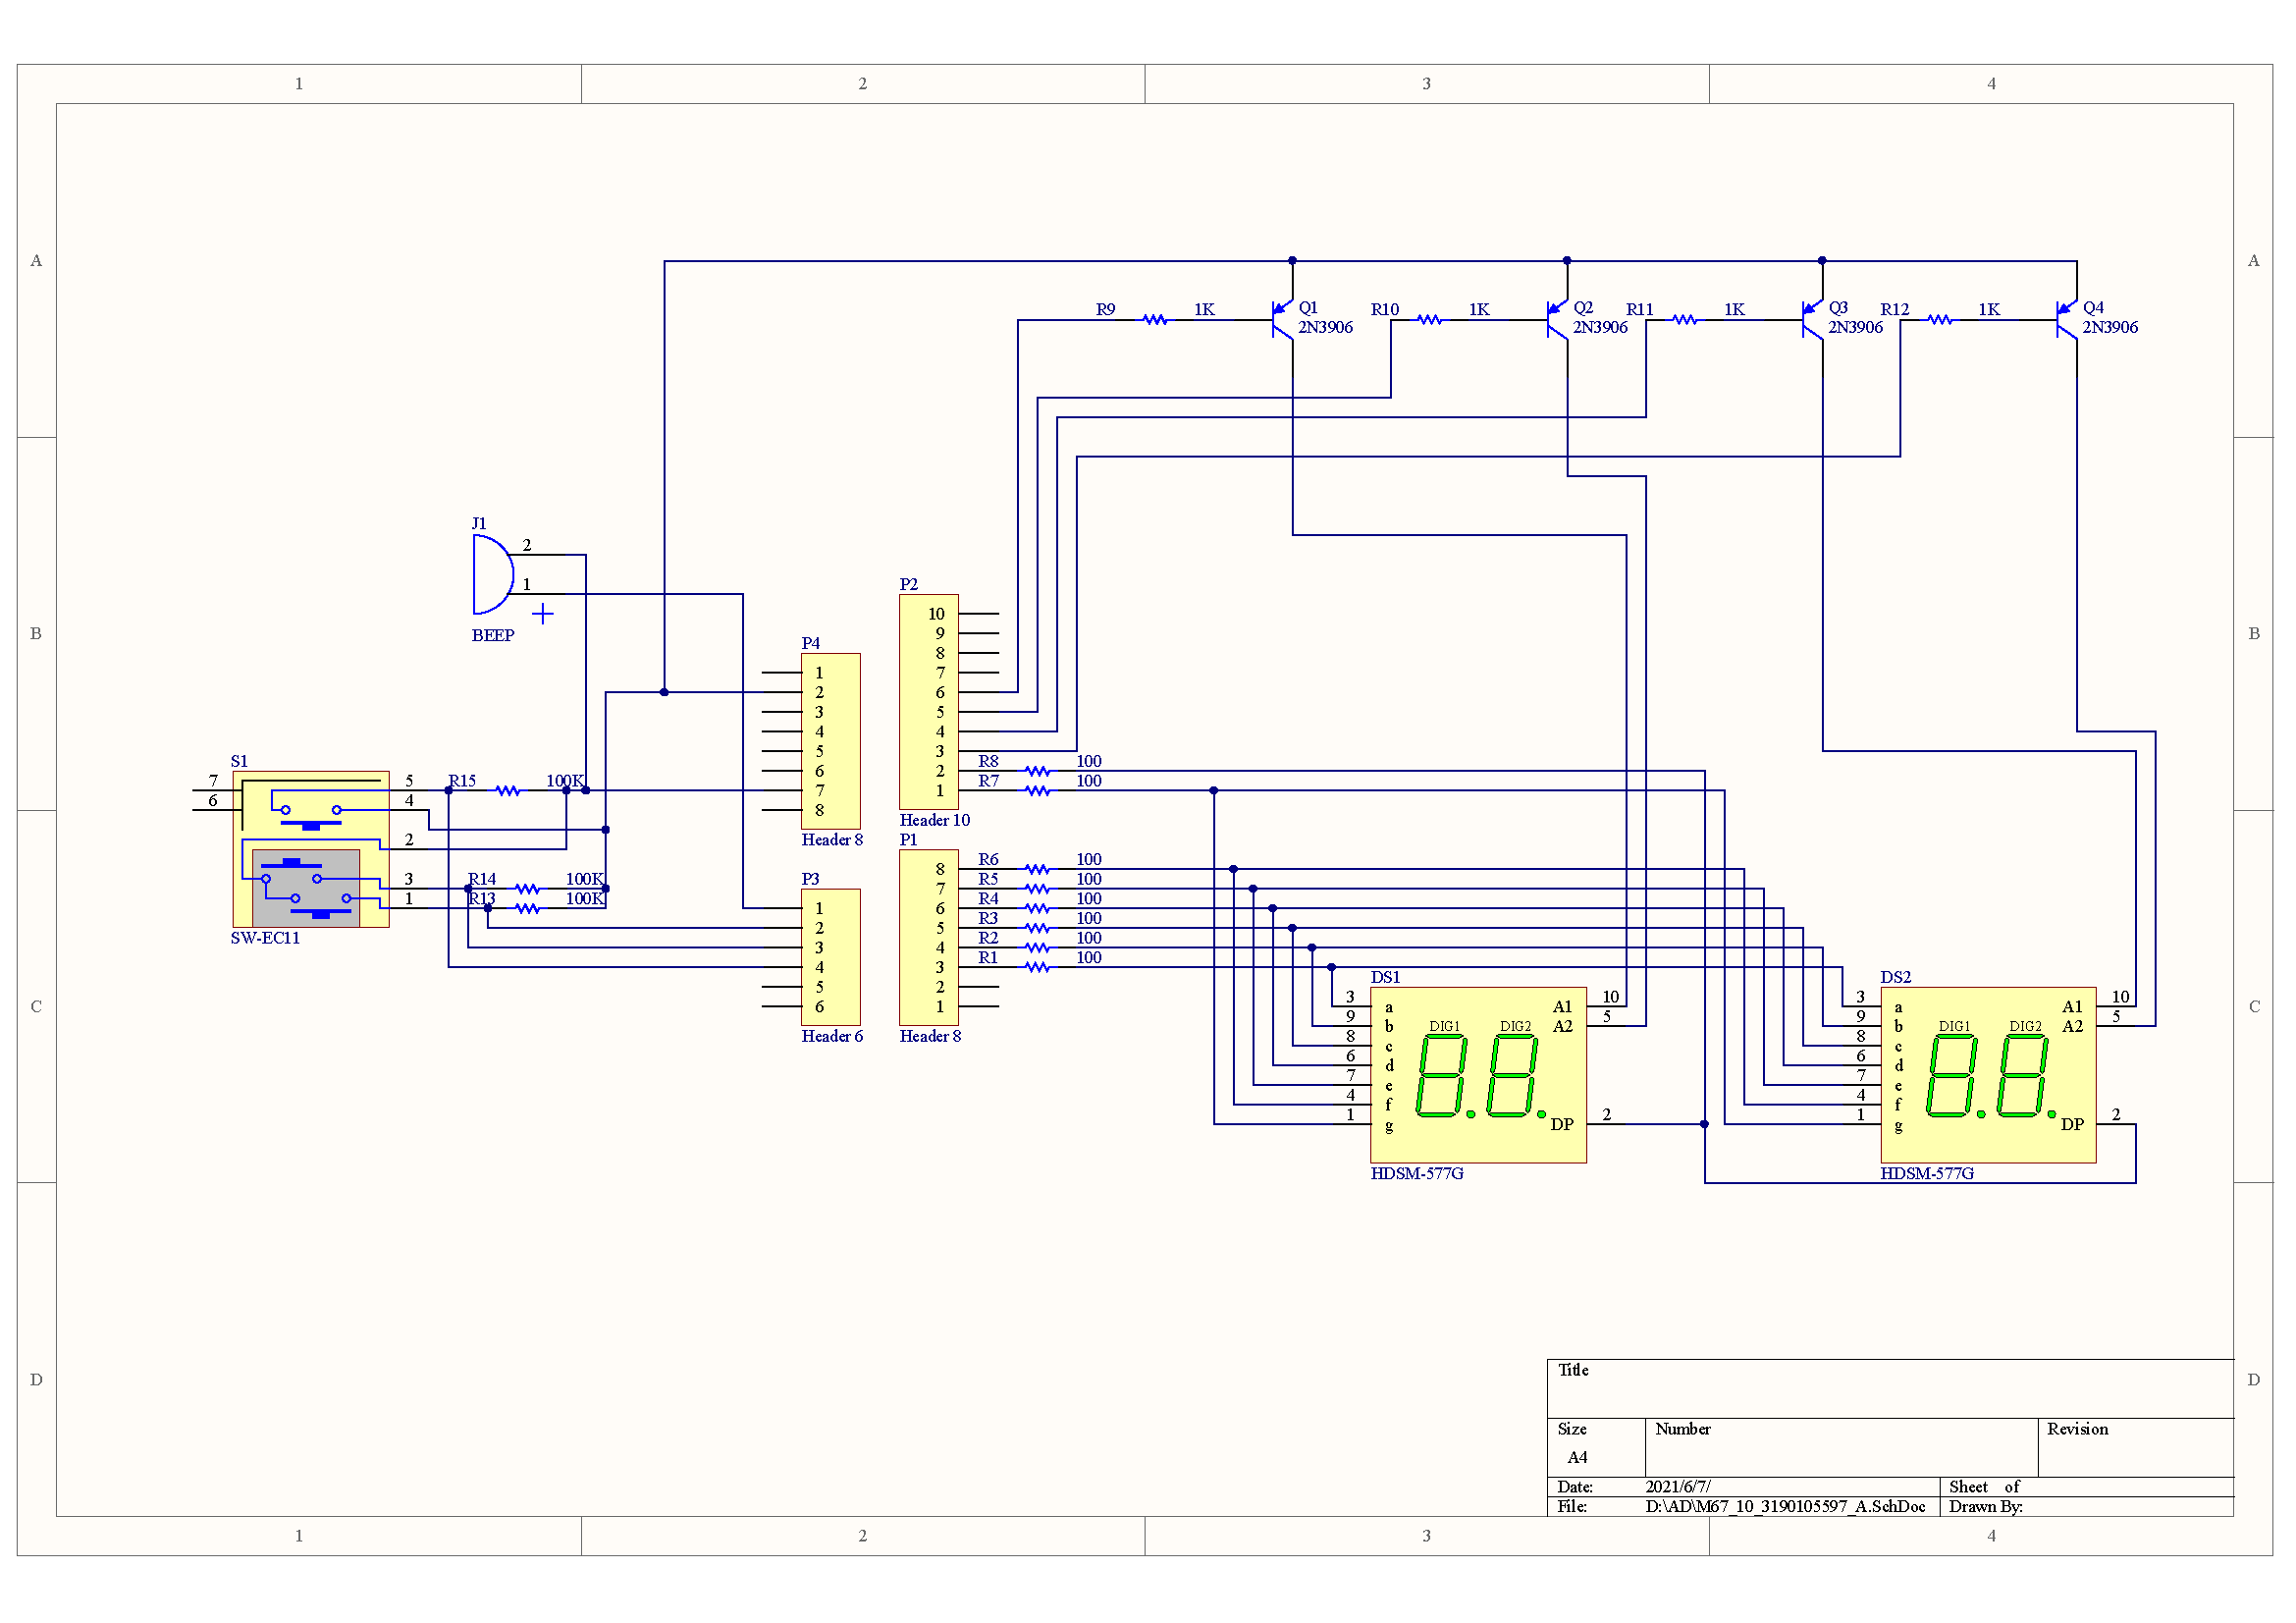
\includegraphics[width = 1\textwidth]{电路图}
                \caption{电路图}
            \end{figure}
            
        \subsection{PCB图}
            \begin{figure}[H]
                \centering
                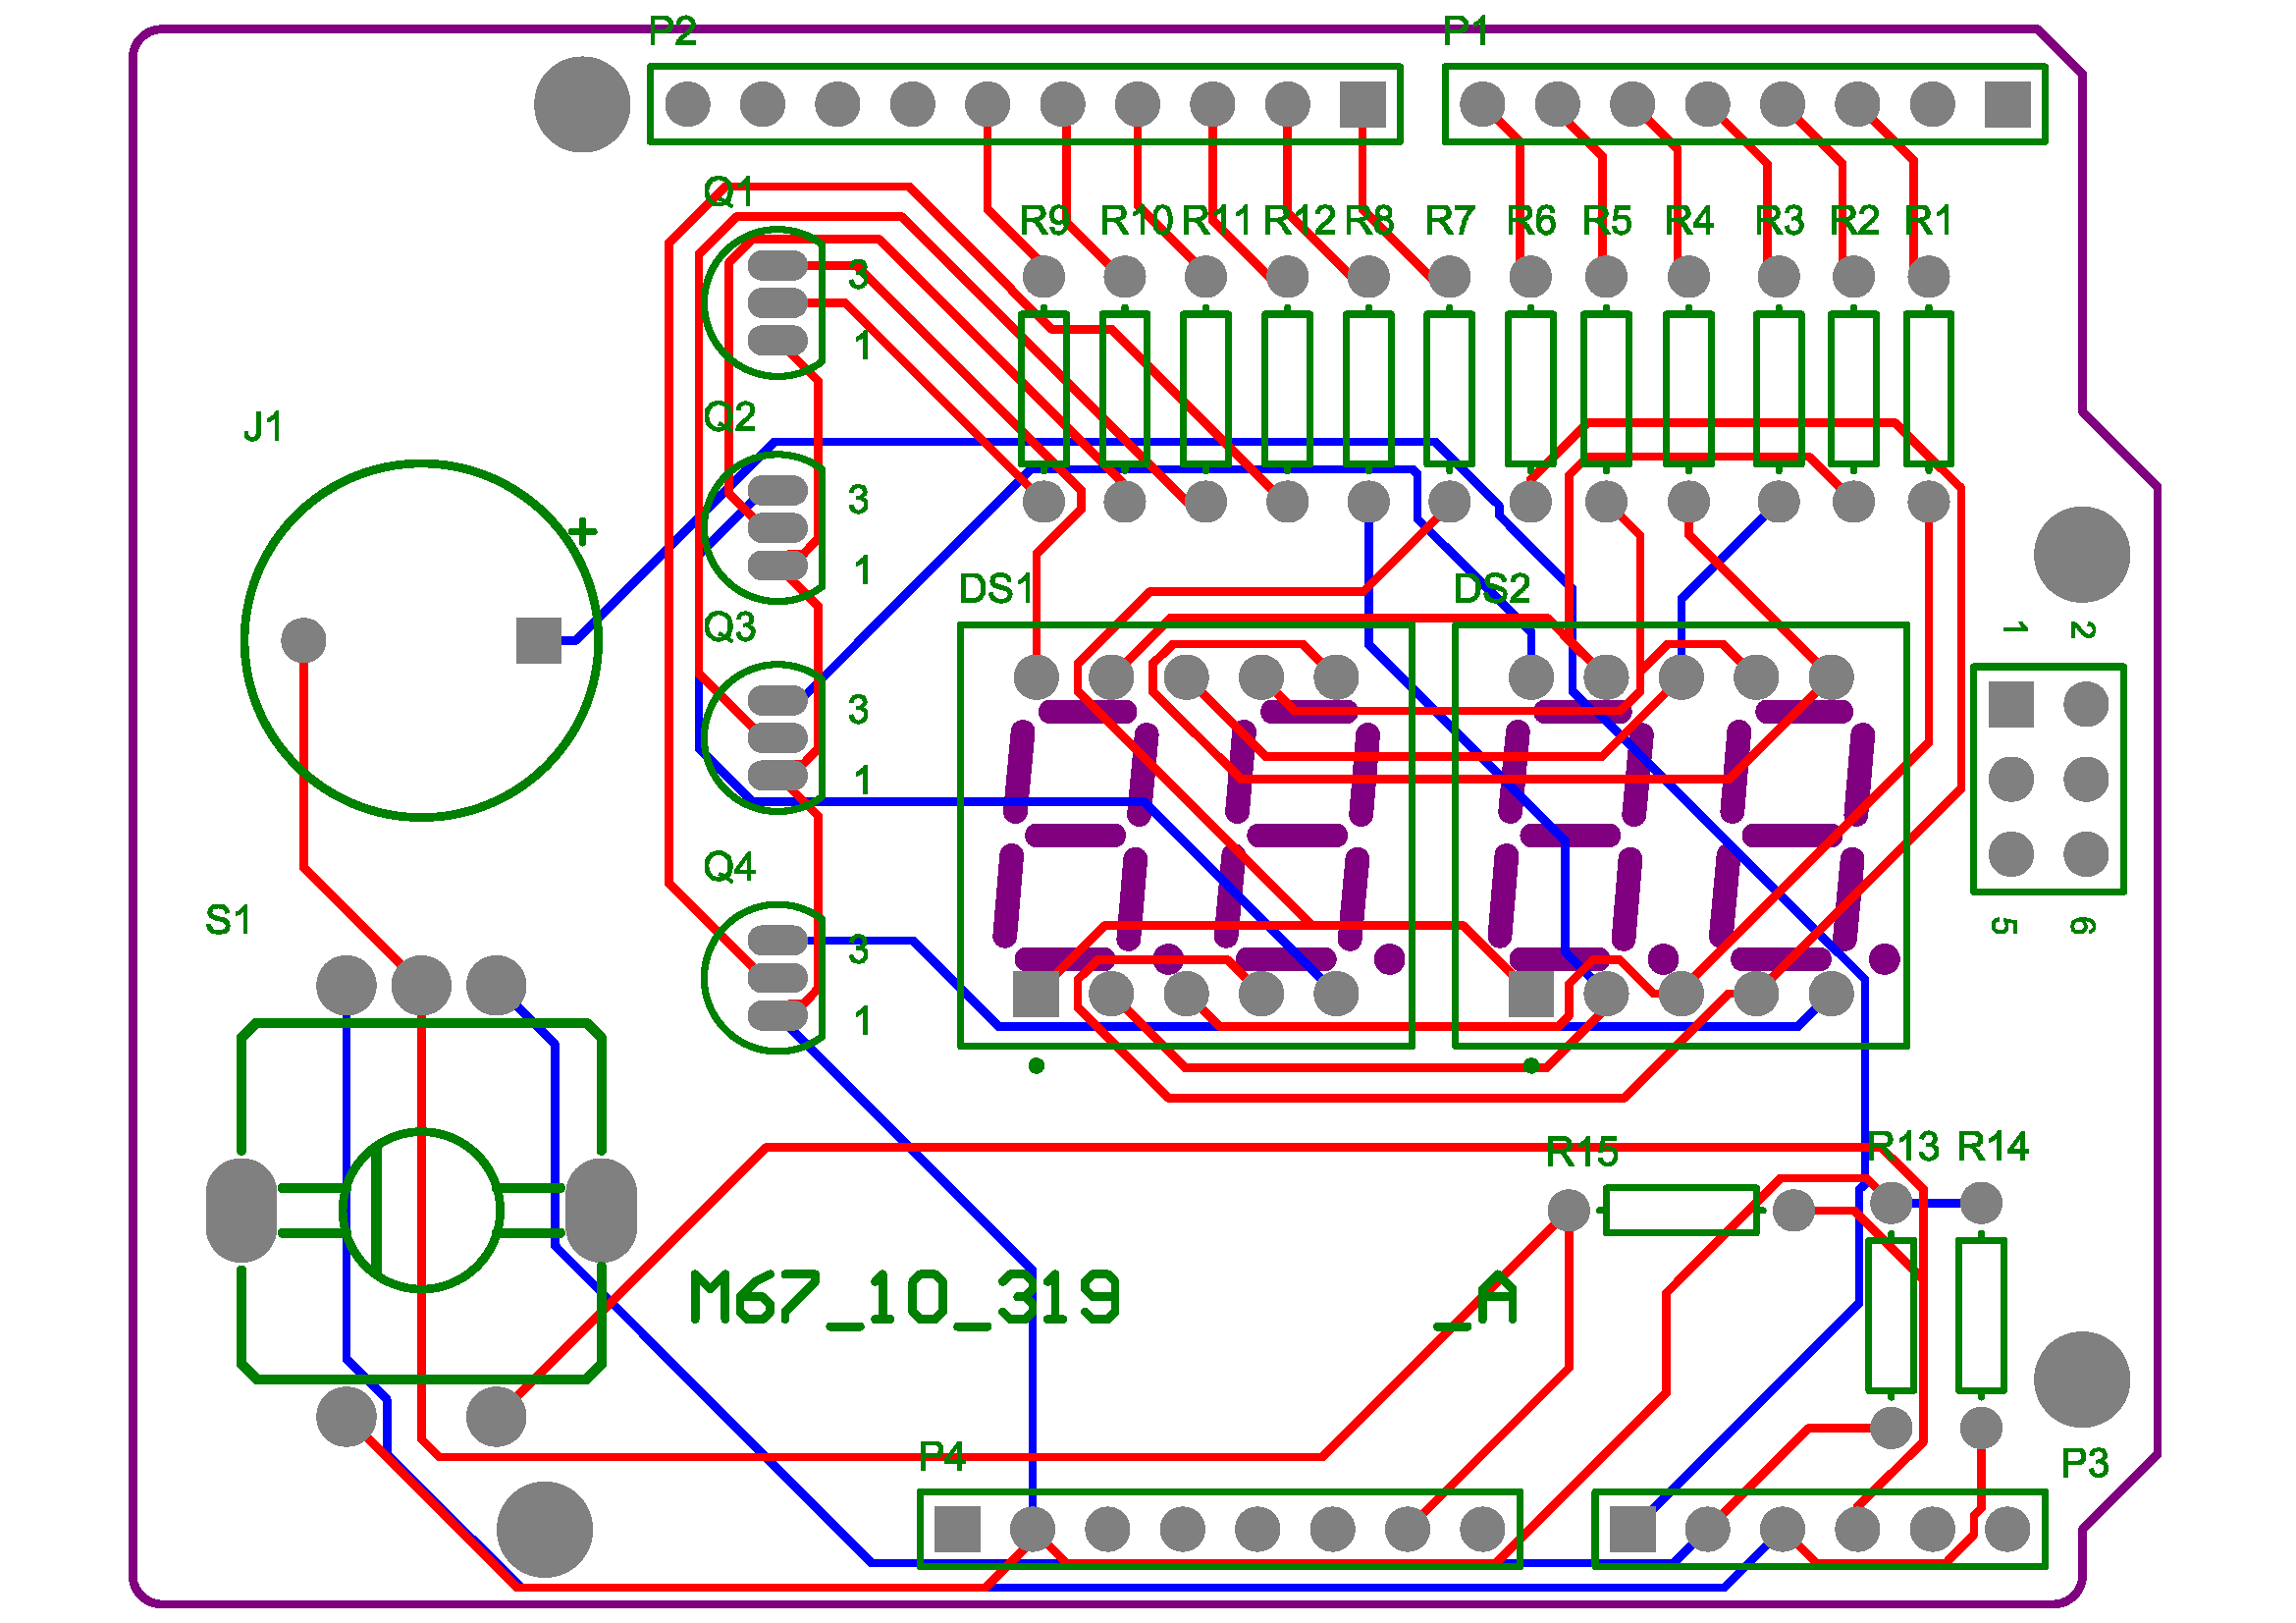
\includegraphics[width = 5in]{PCB}
                \caption{PCB}
            \end{figure}
        
        
        
    
    
\end{document}